\documentclass[10pt]{ctexart}
\usepackage{amsmath,amsfonts,amssymb,amsthm}
\usepackage[a4paper,left=2.5cm,right=2.5cm,top=2cm,bottom=2cm]{geometry}
\usepackage{graphicx,booktabs}
\usepackage{float,bm}
\usepackage{subfigure}
\author{2000012425 张弛}
\title{计算物理第四次作业}
\CTEXsetup[format={\Large\bfseries}]{section}
\newtheorem*{answer}{答}
\newtheorem*{solution}{解}
\newtheorem*{fuck}{证明}
\begin{document}
\maketitle
1.编写最速下降和共轭梯度算法,求解
\begin{align}
    0.05x_1+0.07x_2+0.06x_3+0.05x_4&=0.23,\nonumber\\
    0.07x_1+0.10x_2+0.08x_3+0.07x_4&=0.32,\nonumber\\
    0.06x_1+0.08x_2+0.10x_3+0.09x_4&=0.33,\nonumber\\
    0.05x_1+0.07x_2+0.09x_3+0.10x_4&=0.31.\nonumber
\end{align}
\begin{solution}
    第一个点取
    $$(0,0,0,0)^T.$$
    精度要求取为$10^{-6}$。借助程序"HW4计物第一题.py"得到两种方法的结果
    \begin{table}[H]
        \centering
        \begin{tabular}{ccccc}
            \toprule
            method & 1 & 2 & 3 & 4\\
            \midrule
            SD & 0.9928230 & 1.0043359 & 1.0018034 & 0.9989317\\
            CG & 1.0000000 & 1.0000000 & 1.0000000 & 1.0000000\\
            \bottomrule
        \end{tabular}
        \caption{最速下降法与共轭梯度法的结果}
    \end{table}
    共轭梯度下降法更精确。
\end{solution}
2.利用QR算法、Jacobi算法、Sturm算法+对分法,求下列矩阵的本征值
$$T=
\begin{pmatrix}
    1 & -1 & 0 & 0\\
    -1 & 2 & -1 & 0\\
    0 & -1 & 3 & -1\\
    0 & 0 & -1 & 4
\end{pmatrix}.$$
对于QR算法和Jacobi算法,请写出第$5,10,15,20,\cdots$次迭代后的矩阵$T_k$。对于Sturm序列+对分法请写出
由圆盘定理确定的本征值范围以及第$5,10,15,20,\cdots$次迭代后本征值的近似值。
\begin{solution}
    QR算法是方便的,可以通过施密特正交化和归一化获得正交矩阵$Q$。借助程序"HW4计物第二题QR算法.py"得到
    如下结果。
    $$T_5=
    \begin{pmatrix}
        4.292766 & -0.721314 & 0 & 0\\
        -0.721314 & 3.556114 &  -0.334967 & 0\\
        0 & -0.334967 & 1.896401 & -0.000400\\
        0 & 0 & -0.000400 & 0.254719
    \end{pmatrix}.$$
    $$T_{10}=
    \begin{pmatrix}
        4.734184 & -0.131449 & 0 & 0\\
        -0.131449 & 3.188126 & -0.018582 & 0\\
        0 & -0.018582 &  1.822971 & 0 \\
        0 & 0 & 0 & 0.254719
    \end{pmatrix}.$$
    $$T_{15}=
    \begin{pmatrix}
        4.745079 & -0.017812 & 0 & 0\\
        -0.017812 & 3.177484 & -0.001151 & 0\\
        0 & -0.001151 & 1.822718 & 0 \\
        0 & 0 & 0 & 0.254719 
    \end{pmatrix}.$$
    $$T_{20}=
    \begin{pmatrix}
        4.745278 & -0.002397 & 0 & 0\\
        -0.002397 & 3.177287 & 0 & 0\\
        0 & 0 & 1.822717 & 0 \\
        0 & 0 & 0 &0.254719
    \end{pmatrix}.$$
    其中已经将$10^{-5}$及更小的量写为0。为了写本征值,考虑更高迭代次数的结果。
    $$T_{500}=
    \begin{pmatrix}
        4.745281 & 0 & 0 & 0\\
        0 & 3.177283 & 0 & 0\\
        0 & 0 &1.822717 & 0\\
        0 & 0 & 0 & 0.254719
    \end{pmatrix}.$$
    那么四个本征值分别为
    \begin{table}[H]
        \centering
        \begin{tabular}{ccccc}
            \toprule
            index & 1 & 2 & 3 & 4 \\
            \midrule
            $\lambda$ & 4.745281 & 3.177283 & 1.822717 & 0.254719\\
            \bottomrule
        \end{tabular}
        \caption{QR算法所得本征值}
    \end{table}
    Jacobi算法,认为对所有非对角元都Givens变换一次为迭代一次。借助程序"HW4计物第二题Jacobi算法.py"得到如下结果。
    $$T_5=
    \begin{pmatrix}
        0.254719 & 0 & 0 & 0\\
        0 & 1.822717 & 0 & 0\\
        0 & 0 & 3.177283 & 0\\
        0 & 0 & 0 & 4.745281
    \end{pmatrix}.$$
    $T_{10},T_{15},T_{20}$的结果是一样的。其中已经将$10^{-5}$及更小的量写为0。四个本征值分别为
    \begin{table}[H]
        \centering
        \begin{tabular}{ccccc}
            \toprule
            index & 1 & 2 & 3 & 4 \\
            \midrule
            $\lambda$ & 0.254719 & 1.822717 & 3.177283 & 4.745281\\
            \bottomrule
        \end{tabular}
        \caption{Jacobi算法所得本征值}
    \end{table}
    Sturm算法+对分法。由圆盘定理得到
    $$\alpha=0,\beta=5.$$
    借助程序"HW4计物第二题Sturm.py"得到如下结果。
    \begin{table}[H]
        \centering
        \begin{tabular}{ccccc}
            \toprule
            迭代次数 & 5 & 10 & 15 & 20\\
            \midrule
            & 0.156250 & 0.258789 & 0.254669 & 0.254722\\
            $\lambda$ & 1.718750 & 1.821289 & 1.822662 & 1.822715\\
            & 3.281250 & 3.178711 & 3.177338 & 3.177285\\
            & 4.843750 & 4.741211 & 4.745331 & 4.745278\\
            \bottomrule
        \end{tabular}
        \caption{Sturm算法+二分法所得本征值}
    \end{table}
\end{solution}
3.\textbf{幂次法求矩阵最大模的本征值和本征矢}\ 本题中我们考虑利用幂次法(power mothod)来
求一个矩阵$A\in\mathbb{R}^{n\times n}$的本征值的问题。同时将它运用到一个具体的实例:一维原子链
的振动。

(a)考虑一个一维的原子链的经典振动解,尝试$x(t)=xe^{-i\omega t}$,说明振幅$x\in\mathbb{C}^n$满足本征方程:
$A\cdot x=\lambda x$,本征值$\lambda=\omega^2$。
\begin{solution}
    将$x(t)=xe^{-\omega t}$代入方程
    $$\ddot{x}=-A\cdot x.$$
    得
    $$A\cdot x=\lambda x.$$
    其中
    $$\lambda=\omega^2.$$
\end{solution}
(b)是的,这个题目可以轻易地解析求解。但现在我们假装不知道这点。请写一个利用下面介绍的
幂次法求解上述本征值问题的程序。求出体系最大的本征频率的平方$\omega_{max}^2$,这对应于最大的$\lambda$。
\begin{solution}
    先证明一下幂次法。将初始单位向量$\bm{q^{(0)}}$按本征矢展开
    $$\bm{q^{(0)}}=\sum\limits_{i=1}^{N}s_i\bm{v_i}.$$
    k次迭代结果
    $$\bm{q^{(k)}}=\sum\limits_{i=1}^{N}s_i\lambda_i^k\bm{v_i}.$$
    认为已归一化。可以很明显地看出来
    $$\lim\limits_{k\rightarrow \infty}q^{(k)}=v_1.$$
    那么
    $$\lim\limits_{k\rightarrow \infty}\nu^{(k)}=\lambda_1.$$
    证毕。

    初始单位矢量选择$(1,0,\cdots)$,结果精度控制为$10^{-6}$。借助程序“HW4计物第三题.py”得到如下结果。
    \begin{table}[H]
        \centering
        \begin{tabular}{cccccc}
            \toprule
            $\lambda$ & 1 & 2 & 3 & 4 & 5\\
            \midrule
            3.918979 & 0.121403 & -0.232669 & 0.324579 & -0.389642 & 0.422718\\
            \bottomrule
            \toprule
            6 & 7 & 8 & 9 & 10\\
            \midrule
            -0.421391 & 0.386082 &-0.319917 & 0.228384 & -0.118856\\
            \bottomrule
        \end{tabular}
        \caption{幂次法得到的最大模本征值以及对应本征矢}
    \end{table}
\end{solution}
4.参考课件“常微分方程”中的“洛伦兹吸引子”,重复结果,并额外给出至少2组不同的$\beta,\rho,\sigma$的结果。
$$\begin{pmatrix}
    y_1'\\
    y_2'\\
    y_3'\\
\end{pmatrix}
=\begin{pmatrix}
    -\beta & 0 & y_2\\
    0 & -\sigma & \sigma \\
    -y_2 & \rho & -1 
\end{pmatrix}
\begin{pmatrix}
    y_1\\
    y_2\\
    y_3
\end{pmatrix}.$$
\begin{solution}
    使用普通的欧拉差分向前差商近似。把方程组写出来
    $$\begin{align}
        y_1'&=-\beta y_1+y_2 y_3,\\
        y_2'&=-\sigma y_2+\sigma y_3,\\
        y_3'&=-y_1y_2+\rho y_2-y_3.
    \end{align}$$
    取参数
    $$\beta=\frac{8}{3},\rho=28,\sigma=10.$$
    初始值
    $$x(0)=12,y(0)=4,z(0)=0.$$
    考虑$t\in [0,50]$的运动。步数$10^4$。借助程序"HW4计物第四题.py"得到下图
    \begin{table}[H]
        \centering
        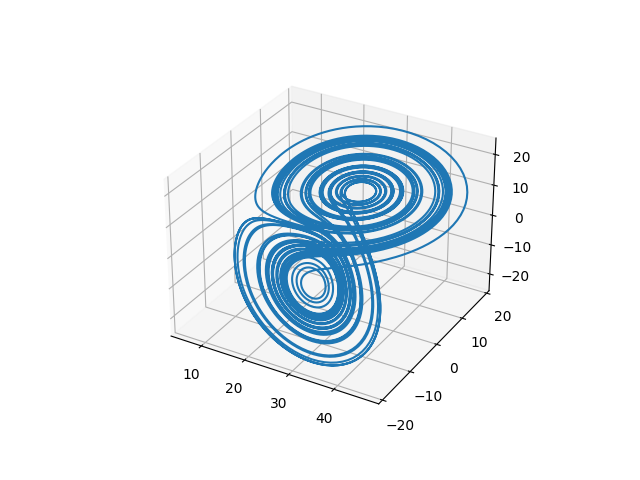
\includegraphics[width=10cm]{1.png}
        \caption{$\beta=\frac{8}{3},\rho=28,\sigma=10$}
    \end{table}
    再考虑参数
    $$\beta=3,\rho=28,\sigma=10.$$
    其余一样,借助程序得到下图
    \begin{table}[H]
        \centering
        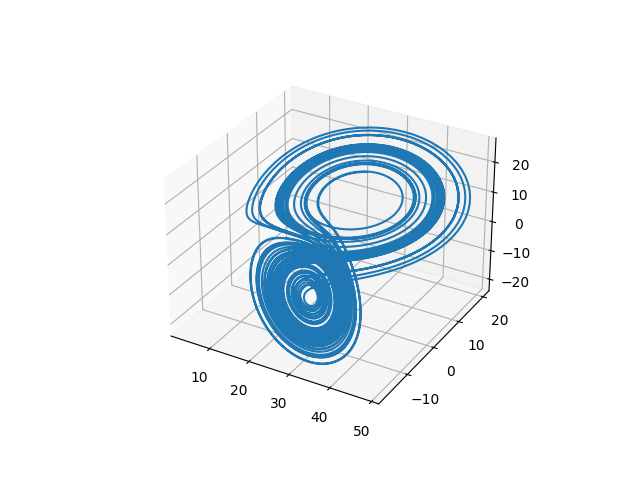
\includegraphics[width=10cm]{2.png}
        \caption{$\beta=3,\rho=28,\sigma=10$}
    \end{table}
    再考虑参数
    $$\beta=\frac{8}{3},\rho=28,\sigma=5.$$
    其余一样,借助程序得到下图
    \begin{table}[H]
        \centering
        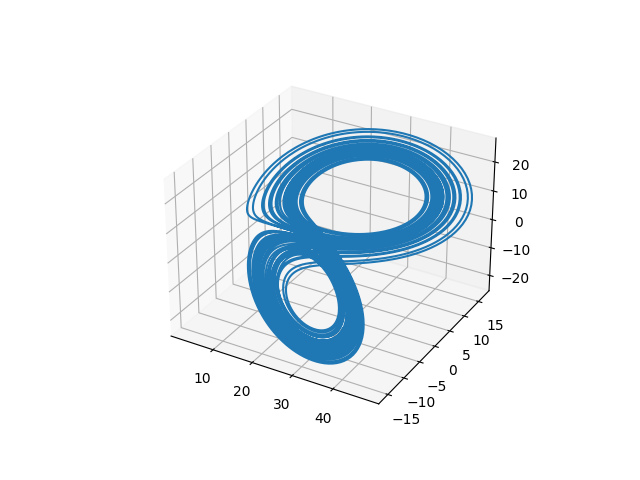
\includegraphics[width=10cm]{3.png}
        \caption{$\beta=\frac{8}{3},\rho=28,\sigma=5$}
    \end{table}
\end{solution}
\end{document}